\documentclass[12pt,a4paper]{article}
\usepackage[utf8]{inputenc}
\usepackage[brazil]{babel}
\usepackage[table]{xcolor}
\usepackage{graphicx}
\usepackage{color}
\usepackage{hyperref}
\usepackage{abnt-alf}
\usepackage[top=3cm,bottom=2cm,left=3cm,right=2cm]{geometry}
\usepackage{indentfirst}
\usepackage{float}

\begin{document}

% CAPA
\pagestyle{empty}
\begin{center}
\large  \textbf{UNIVERSIDADE PRESBITERIANA MACKENZIE}
\large  \textbf{PROGRAMA DE PÓS-GRADUAÇÃO EM}\\
\large  \textbf{ENGENHARIA ELÉTRICA E COMPUTAÇÃO}\\
\vskip 2.0cm
\textbf{\large Fernando Cainelli Tolentino}\\
\vskip 4.0cm
\setlength{\baselineskip}{1.5\baselineskip}
\textbf{\large Latent Dirichlet Allocation: Visualizando e Explorando Documentos}\\
\vskip 4.5cm
\end{center}
\hfill{\vbox{\hsize=8.5cm\noindent\strut
Projeto de Pesquisa apresentado ao Programa\break
de Pós-Graduação em Engenharia Elétrica e\break
Computação da Universidade Presbiteriana\break
Mackenzie como parte dos requisitos para a\break
aprovação na disciplina de Metodologia do\break
Trabalho Científico.}\\
\strut}
\vskip 3.0cm
\textbf{\normalsize Orientador: Prof. Dr. Leandro Augusto da Silva}\\
\vskip 2.0cm
\begin{center}
São Paulo\\
2017\\
\end{center}

% RESUMO
\newpage
\thispagestyle{plain}
\pagenumbering{roman}
\begin{center}
\large
\textbf{RESUMO}
\end{center}
\renewcommand{\baselinestretch}{0.6666666}
Latent Dirichlet Allocation(LDA) é um modelo generativo probabilistico que sumariza uma coleção de documentos em tópicos além de apresentar a relevância de cada tópico a cada
 documento. A interpretação e exploração de uma coleção de documentos pelo LDA pode ser feita a nível de tópico, palavra ou documento. LDAvis é um sistema para
 exploração de tópicos e palavras resultantes do modelo LDA, esse trabalho tem como objetivo extender as suas funcionalidades para exploração do modelo a nível de documento e relações de redes,
 promovendo uma ferramenta de busca aprimorada em um corpus.


% \begin{flushleft}
% {\bf Palavras-chave:} {\it apresentação, separada por vírgulas, de três a seis unitermos significativos para o trabalho.}
% \end{flushleft}

% SUMÁRIO
\newpage
\thispagestyle{empty}
\tableofcontents

% DESENVOLVIMENTO
\newpage
\pagestyle{plain}
\pagenumbering{arabic}
\renewcommand{\baselinestretch}{1.5}
\normalsize
\section{INTRODUÇÃO}
 Neste trabalho, consideramos o problema de visualização de modelos de tópicos, em particular Latent Dirichlet Allocation,\cite{blei2003latent}.
 Propomos um aprimoramento da aplicação LDAVis de \citeonline{sievert2014ldavis} para explorar documentos e suas relações. Mostramos que em uma base de dados
 com documentos contendo metadados e relações de rede, como artígos científicos ou e-mails por exemplo, é possível realizar a busca aprimorada de documentos além de identificar
 comunidades de redes de sociais através de interesse comum segundo os tópicos criados pelo modelo LDA.

 A estrutura organizacaional dessa dissertação consiste em 5 capitulos. O capítulo 1, segue com uma breve introdução e organização do trabalho. 
  No capítulo 2, justificamos a elaboração do trabalho demonstrando que a visualização de modelos de tópicos é uma das áreas em carência de pesquisa atualmente, 
  e como esse trabalho busca contribuir com o campo de \textit{Information Retrival} para modelos de tópicos. No capítulo 3, discorremos sobre o referencial teórico presente, 
  é detalhado o funcionamento do modelo probabilístico LDA além da apresentação do algorítmo K-Means como base de comparação. No capítulo 4, mostramos a metodologia adotada, 
  a arquitetura, o processo de mineração de dados, as justificativas de adoção de cada parâmetro livre na criação do modelo além das funcionalidades propostas para
  aplicação de busca. Por fim, no capítulo 5, apresentamos o cronograma com as tarefas pendêntes para a conclusão do trabalho.


% JUSTIFICATIVA
\section{JUSTIFICATIVA}
Com acúmulo cada vez mais crescente de informações digitalizadas e armazenadas na forma de: artigos, blogs, jornais, e-mails, livros, mensagens instantâneas, redes sociais, entre outros, 
 a tarefa de organizar, indexar e buscar essas informações é fundamental. Para possibilitar usuários navegar por esses documentos e encontrar a informação desejada, utilizamos hoje dois métodos principais, 
 links e busca. Links correlatam trechos de um documento a outro, são muito úteis pois possibilitam uma extensão da leitura e aprofundamento do conhecimento,
 direcionando o leitor a termos ou assuntos relacionados de alguma forma ao documento original. Apesar de ser uma ótima maneira de fornecer conteúdo diretamente relacionado,
 encontramos desafios na aplicação em escala, pois muitas vezes, essa ferramenta  é implementada de forma manual pelo o autor. A busca por outro lado,
 requer um processo que pode ser automatizado de forma efetiva, pois quando informações presentes nos documentos são indexadas, é permitido ao usuário procurar um documento por palavra chave ou metadados presentes nele.
 Esse processo é muito disseminado, e motores de busca utilizam de técnicas sofisticadas em diversas áreas como ranqueamento de resultados e similaridade de palavras para melhorar essa experiência.
 O trabalho de \citeonline{mikolov2013efficient} por exemplo, possibilita em escala, fornecer funcionalidades como sugestões de termos de pesquisa baseado na ordem das palavras digitadas além de extensão de busca utilizando termos similares.

Essas técnicas são poderosas para interagirmos com nossos documentos, no entanto há uma lacuna, imagine explorar documentos por meio de temas de interesse específico,
 visualizar as palavras mais relevantes em cada tema e explorar os documentos com a usabilidade de um mapa, com possibilidade de zoom in, zoom out, além de visualizar a relação entre documentos de uma maneira intuitiva,
 por proximidade. Essa, pode ser uma forma complementar de busca aos métodos citados no parágrafo anterior. A aplicação desse método pode ser em qualquer corpus, no entanto, como exemplo,
 vamos demonstrar como aplicação em um corpus contendo documentos de e-mail. E-mails possuem informações que podem aprimorar ainda mais a experiência de exploração,
 pois os documentos podem ser exibidos em forma de nós, conectando remetentes a destinatários e aprimorando ainda mais a exibição dos resultados da pesquisa.

Pesquisas apontam que em 2017 atingiremos uma média de 269 bilhões de e-mails enviados e recebidos diariamente, e é esperado continuar a crescer a uma taxa média de 4.4\% ao ano nos próximos quatro anos,
atingindo 319.6 bilhões ao final de 2021 \cite{radicati2017}.

\begin{table}[h]
  \centering
  \begin{tabular}{l*{6}{c}r}
  &					2017 &	2018 &	2019 &	2020 &	2021 & \\
  \hline
  Quantidade de E-mails &			269.0 &	281.1 &	293.6 &	306.4 &	319.6 & \\
  Crescimento(\%) &  	&		4.5\% &	4.4\% &	4.4\% &	4.3\% & \\
  \hline
  \end{tabular}
  \caption{Tráfego de Email Mundial Diário  (Bi). \cite{radicati2017}}
\end{table}

A taxa de crescimento da quantidade de mensagens enviadas e recebidas impressiona, não só por se tratar de uma técnologia dos anos 70,
mas principalmente pela forte adoção de novos recursos de comunicação como: mensagem instantânea, redes sociais, videoconferência, chat, etc. A comunicação via e-mail permanece sólida principalmente em empresas,
estas, por sua vez, tem a necessidade de aplicar a inteligência nos negócios para manter-se competitivas. O Business Intelligence deve ser utilizado não só em escopos diretamente relacionados ao negócio,
como clientes, produtos, etc. mas também nos indiretos, como colaboradores, buscando obter insights, melhoria dos processos e otimização.
Frequentemente, e-mails são deixados fora da equação pela falta de ferramentas específicas e complexidade em tratar dados não estruturados,
neste artigo, queremos promover um método complementar de exploração de documentos, para isso,
vamos utilizar um conjunto de documentos de e-mail de uma empresa e fazer uso do modelo generativo probabilístico proposto por \citeonline{blei2003latent}, Latent Dirichlet Allocation,
além de técnicas de processamento e visualização de conhecimento. Faremos uso das mesmas técnicas, na análise exploratória do conjunto de dados,
espera-se também obter informações relevantes que possam ser utilizadas na compreensão do negócio da empresa.

% REFERENCIAL TEÓRICO
\section{REFERENCIAL TEÓRICO}
No campo de processamento de linguagem natural e recuperação de informação, existem diversas técnicas de agrupamento, análise e extração de sentido de um conjunto de dados de textos.
 Nesta seção, vamos apresentar as técnicas disponíveis e trabalhos relatos relevantes utilizados neste artigo.



% K-MEANS
\subsection{K-MEANS}
O algoritmo K-Means, assinala a cada objeto de um conjunto de dados à um grupo, foi introduzido inicialmente por \citeonline{macqueen1967some} e é um dos algoritmos mais estudados na literatura.
 O algoritmo é inicializado com dois parâmetros principais, o número de clusters, ou grupos, disponíveis para os objetos no dataset serem classificados e um vetor de objetos que representa o conjunto de dados.
 Cada objeto no conjunto de dados pode ser assinalado à um grupo a cada iteração. Primeiro determinamos os centróides iniciais,
 centróides são a representação de um grupo e seu valor é dado pela média dos objetos desse grupo, são iniciados randomicamente, como proposto  pelo trabalho original,
 ou utilizando algum algoritmo de otimização, em alguns casos, o K-Means pode convergir para grupos distintos dependendo do valor inicial dos centróides. 
 Existem diversos estudos que adotam diferentes algoritmos e técnicas para inicialização dos centróides,
 \citeonline{yuan2004new} propuseram um método para se obter os centróides iniciais de acordo com a distribuição do conjunto de dados,
 em sua pesquisa obtiveram melhor acurácia com essa técnica quando comparada a inicialização randômica proposta no trabalho original de \citeonline{macqueen1967some}.

O próximo passo é rodar o algoritmo até que convirja. Para cada iteração,
 o algoritmo assinala cada objeto ao grupo cujo centróide está mais próximo e calcula a nova média do grupo para então ajustar os valores dos centróides.
 Para determinar a distância entre um objeto observado e os centróides, K-Means utiliza a distância Euclidiana que calcula a diferença entre um objeto vetor \(X=(x_1, x_2... x_n)\) 
 e um centróide vetor \(C=(c_1, c_2... c_n)\) com a seguinte fórmula: 

\begin{equation}
d(X,C) = \sqrt{(x_1 - c_1)^2 + (x_2 - c_2)^2 ... + (x_n - c_n)^2}
\end{equation}

O objeto $X$ será assinalado ao grupo cujo centróide tem a menor distância Euclidiana. Em seguida, o algoritmo percorre cada grupo calculando a média dos objetos nele presente,
 e define esse valor ao centróide do grupo. O processo se repete até que os objetos não troquem de grupo.

O algoritmo K-Means assinala cada objeto do conjunto de dados a exatamente um grupo, no entanto, para problemas que objetos podem pertencer a mais de um grupo,
 ou quando grupos de dados são representados por uma forma não circular, uma vez que é  utilizada a distância Euclidiana para assinalar objetos a grupos, um modelo misto, ou mixture model,
 podem obter agrupamentos com melhores representações.



%% LATENT DIRICHLET ALLOCATION
\subsection{LATENT DIRICHLET ALLOCATION}
Latent Dirichlet Allocation, ou LDA, é um modelo generativo probabilístico proposto por \citeonline{blei2003latent}, esse modelo é usado em diversas áreas como análise de sentimento,
 classificação de documentos, bioinformática, agrupamento de dados entre outros. LDA sugere que palavras carregam uma forte informação semântica,
 e que documentos com assuntos similares contém também um grupo de palavras similares. Os tópicos latentes, ou ocultos,
 são portanto descobertos identificando o grupo de palavras no corpus que co-ocorrem frequentemente dentro dos documentos. A idéia básica do LDA é:

\begin{enumerate}
  \item Cada documento é representado por uma mescla de tópicos.
  \item Cada tópico é formado por uma distribuição de palavras.
\end{enumerate}

LDA encontra o modelo probabilístico de um conjunto de dados. Enquanto modelos como os de Mistura de Unigramas, assumem que cada documento exibe características de apenas um tópico,
 o modelo do LDA  permite que documentos contenham múltiplos tópicos ao mesmo tempo e com relevância distintas. Nesta seção, vamos discorrer sobre as principais características do trabalho original de \citeonline{blei2003latent}.
 A pesquisa de \citeonline{hu2009latent} foi complementar durante essa seção para melhor compreender o trabalho original.

Antes de nos aprofundarmos na descrição do algoritmo, façamos uma introdução da terminologia formal e notações usada nesta seção.

\begin{enumerate}
  \item Uma $palavra$ é a mais básica unidade de dado, definida com um item de um vocabulário indexado por \(w \in \{1,. . . , V\}\)  , onde $V$ é o número de palavras únicas dentro de um corpus, também denominado vocabulário. Palavras são representadas como um vetor de base unitária.
  \item Um documento é uma sequência de $N$ palavras denotadas por \(\textbf{ w} = (w_1, w_2,. . . ,  w_N)\).
  \item Um corpus é uma coleção de $M$ documentos denotados por \(\textbf{ D} = \{\textbf{ w}_1, \textbf{ w}_2, . . ., \textbf{ w}_M\}\).
\end{enumerate}



%% PROCESSO GENERATIVO
\subsection{PROCESSO GENERATIVO}
O LDA assume que documentos são criados via um processo generativo no qual palavras nos documentos são geradas. Dado o tamanho do documento,
 nós escolhamos uma mistura de tópicos usando a distribuição multinomial de tópicos para escolher as palavras que devem ser usadas para preencher a cota de cada tópico. ex:
 Temos um grupo de artigos que assumimos que tais artigos podem ser classificados em quatro tópicos, Esportes, Animais, Tecnologia e Artes, cada tópico pode ser definido pela seguinte lista de palavras:

\begin{itemize}
  \item \textbf{ Esportes:} bola, futebol, basquete, gol, pontos, corrida, natação.
  \item \textbf{ Animais:} coelho, cachorro, gato, galinha, touro, aranha.
  \item \textbf{ Tecnologia:} computadores, smartphone, tablet, tech, câmera, web.
  \item \textbf{ Artes:} cinema, dança, música, canção, pintura, cores, movimento, instrumento.
\end{itemize}

Com as informações apresentadas acima, queremos gerar um novo artigo que contenha 75\% artes e 25\% esporte, primeiro determinamos o tamanho do artigo em número de palavras,
 então para cada tópico escolhido para mistura, selecionamos as palavras de cada tópico proporcionalmente a ele. 
 O LDA usa esse conceito de forma reversa para determinar a distribuição de tópicos por documento e a distribuição de palavras por um tópico. 
 O processo generativo permite diferentes graus de relevância de uma palavra em um tópico, e um tópico em um documento, na teoria da probabilidade isso é chamado permutabilidade,
 ou exchangeability \cite{aldous1985exchangeability}. O processo generativo pode ser descrito formalmente como:

Para cada documento indexado por $d \in \{1,. . . , M\}$ em um corpus $D$:

\begin{enumerate}
  \item Escolha um vetor de tópico $\theta _d$ de dimensão $K$ da distribuição $p(\theta|\alpha)=Dirichlet(\alpha)$.
  \item Para cada uma das $N$ palavras($w_n$) dentro de um documento:
  \begin{enumerate}
  	\item Escolha um tópico \(z_n \in \{1,. . . , K\}\) do Multinômio($\theta$).
    \item Escolha uma palavra $w_n$ de \(p(w_n=1| z_n=j,\beta)=\beta _{ij}\), que é a distribuição probabilistica multinomial condicionada ao tópico $z_n$.
  \end{enumerate}
\end{enumerate}

O  hiper parâmetro $\alpha$ é um vetor de dimensão $K$ com itens \(\alpha _i>0\) e é uma distribuição Dirichlet priori da distribuição de tópicos por documento,
 o hiper parâmetro $\beta$ é uma distribuição Dirichlet priori da distribuição de palavras por tópicos. $\theta _d$ é a distribuição de tópicos para o documento $d$. $Z_{dn}$ e $W_{dn}$ são as variáveis a nível de palavras e são amostradas uma vez para cada palavra em cada documento.

Uma variável de distribuição Dirichlet randômica $\theta$ com dimensão $K$ tem como propriedade: $\theta ^i \geq 0, \displaystyle\sum_{i=1}^{K} \theta ^i = 1$ e têm a seguinte densidade probabilística:

\begin{equation}
p(\theta|\alpha) = \frac{\Gamma(\displaystyle\sum_{i=1}^{K} \alpha _i)}{\displaystyle\prod_{i=1}^{K} \Gamma(\alpha _i)} \theta _1 ^{\alpha _i - 1} ...  \theta _K ^{\alpha _K - 1}
\end{equation}

A distribuição Dirichlet é utilizada pois possui um conjunto de propriedades importantes que possibilitam um processo de inferência e estimação de parâmetros mais simples.
 A distribuição é da família exponencial, conjuga com a distribuição multinomial, possui dimensões finitas e possui estatística suficiente.
 A distribuição  acima dá a cada documento seu próprio vetor de distribuição que indica a relevância de cada tópico $K$ para com aquele documento.
 O processo generativo descrito acima define a distribuição conjunta para cada documento $\textbf{ w}_d$.

Dado os hiper parâmetros $\alpha$ e $\beta$, a distribuição conjunta de uma mistura de tópico $\theta$ e um conjunto de $N$ tópicos $z$ é dado por:

\begin{equation}
p(\theta,\textbf{z},\textbf{w}|\alpha,\beta) = p(\theta|\alpha) \prod_{n=1}^{N} p(z_n|\theta)p(w_n|z_n,\beta)
\end{equation}


A Figura 1 ilustra o Plate Notation do modelo LDA, as caixas são pratos representando réplicas,
 o $M$ denota o número de documentos que é associado ao prato externo e o interno representa as palavras dentro de um documento, onde $N$ denota o número de palavras.

\begin{figure}[H]
	\centering
    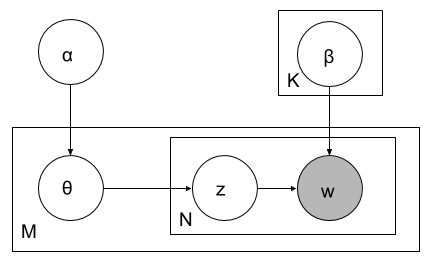
\includegraphics[height=10cm]{images/figure_1.png}
    \caption{Plate Notation representando o modelo LDA, adaptado de \citeonline{blei2003latent}}
\end{figure}

onde $p(z_n | \theta)$é simplesmente $\theta _i$ para cada $i$ único, tal que $z_{ni}=1$. Nós obtemos a distribuição marginal de um documento $d$ integrando sobre $\theta$ e somando sobre $z$.

\begin{equation}
p(\textbf{w}|\alpha,\beta)=\int{p(\theta|\alpha)\Bigg(\prod_{n=1}^{N}\sum_{z_n} p(z_n|\theta)p(w_n|z_n,\beta)\Bigg)d\theta}
\end{equation}

A probabilidade de um corpus é obtida com o produto das probabilidades marginais de um documento:

\begin{equation}
p(D|\alpha,\beta)= \prod_{d=1}^{M} \int{p(\theta _d|\alpha)\Bigg(\prod_{n=1}^{N_d}\sum_{z_{dn}} p(z_{dn}|\theta _d)p(w_{dn}|z_{dn},\beta)\Bigg)d\theta _d}
\end{equation}



%% INFERÊNCIA
\subsection{INFERÊNCIA}
A Eq.(3) foi baseada nos hiper parâmetros antecedentes $\alpha$ e $\beta$, nesta seção, nós descrevemos o procedimento para inferência.

O problema de inferência principal a se resolver é o de se computar a distribuição posteriori das distribuições latentes:

\begin{equation}
p(\theta,\textbf{z}|\textbf{w},\alpha,\beta) = \frac{p(\theta,\textbf{z},\textbf{w}|\alpha,\beta)}{p(\textbf{w}|\alpha,\beta)}
\end{equation}

A distribuição acima é intratável de se computar em geral, o numerador é a distribuição conjunta das variáveis randômicas, que são computáveis para qualquer configuração de variáveis ocultas,
 o denominador é a distribuição marginal, em teoria, pode ser calculada somando a distribuição conjunta de todas instâncias possíveis, no entanto,
 o número de estruturas de tópicos é exponencial e essa soma é intratável de se computar \cite{blei2012probabilistic}. Para normalizar a distribuição da Eq.(4) é utilizado a distribuição marginal,
 de todos os documentos em um corpus:

\begin{equation}
p(\textbf{w}|\alpha,\beta)=\frac{\Gamma(\sum_{i}\alpha_i)}{\prod_{i}\Gamma(\alpha_i)}\int{\Bigg(\prod_{i=1}^{K}\theta_i^{\alpha_i-1}\Bigg)} \Bigg(\prod_{n=1}^{N}\sum_{i=1}^{K}\prod_{j=1}^{V}(\theta_i\beta_{ij})^{w_n^j}\Bigg)d\theta
\end{equation}

Embora a distribuição posterior é intratável devido ao acoplamento do $\theta$ e $\beta$, existe uma variedade de algoritmos de aproximação de inferência que podem ser usados,
 os métodos comumente encontrados na literatura são baseados em amostragem ou variação.

O algoritmo de amostragem mais comum para modelação de tópicos é o Gibbs Sampling, uma instanciação especial da Cadeia de Markov Monte Carlo (MCMC) \cite{jordan1999introduction},
 uma sequência de variáveis randômicas, uma dependente da anterior. O algoritmo roda coletando amostras da distribuição assintótica e então aproximando a distribuição com as amostras coletadas.
 O problema reside em não saber ao certo  quando o algoritmo convergiu para solução, além dos seus requisitos de memória, já que escala linearmente com o número de palavras em um corpus,
 isso torna o algoritmo não adotável em uma conjunto de dados muito grande \cite{vrehuuvrek2011scalability}.

O método mais utilizado em modelos de variável latente é o algoritmo variacional Expectation-Maximization(EM), que permite a estimação de parâmetros não supervisionada de maneira computacionalmente eficiente,
 o método determinístico de aproximação EM resulta em uma estimativa tendenciosa. Em cada iteração é atualizado os parâmetros computando os valores esperados das variáveis sobre a distribuição posterior na Eq.(7).


\begin{figure}[H]
	\centering
    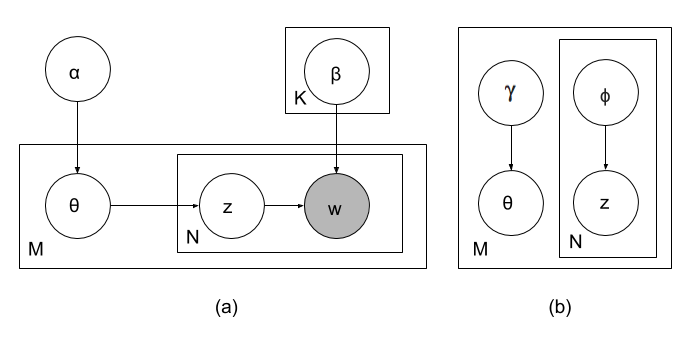
\includegraphics[height=10cm]{images/figure_2.png}
    \caption{(a) Representação gráfica do modelo LDA. (b) A aproximação variacional para a distribuição posteriori. Adaptado de \citeonline{blei2003latent}}
\end{figure}

A ideia do trabalho original de utilizar inferência variacional baseada na convexidade é de se fazer o uso da desigualdade de Jensen para obter um limite inferior ajustável na verossimilhança \cite{jordan1999introduction} onde os parâmetros variacionais são escolhidos através de um processo de otimização,
 tentando encontrar o limite inferior mais próximo em cada iteração. Considerando a Figura 2(a), a problemática do acoplamento dos parâmetros $\theta$ e $\beta$ surge devido às bordas entre $\theta$, $z$,
 e nó $w$, removendo-os, as dependências entre as variáveis que tornam a equação intratável também são removidas. Com isso,
 acabamos com um Plate Notation simplificado com parâmetros variacionais livres ilustrados na Figura 2(b), obtendo a família de distribuição de probabilidade nas variáveis ocultas,
 que é caracterizada pela seguinte distribuição variacional:

\begin{equation}
q(\theta,\textbf{z}|\gamma,\phi)=q(\theta|\gamma)\prod_{n=1}^{N}q(z_n|\phi_n), 
\end{equation}

onde a distribuição  $q(\gamma|\phi)$ é a distribuição Dirichlet com parâmetro variacional $\gamma_d$ mostrando a distribuição dos tópicos em cada documento.
 As distribuições $q(z_n | \phi_n)$ são multinomiais com parâmetros variacionais $\phi_n$ e existem a nível de palavras, onde $\phi_{ni}$ é a probabilidade que a $n_{gesima}$ palavra foi gerada pelo $i_{gesimo}$ tópico oculto.

O próximo passo é configurar um problema de otimização que determina os parâmetros $\gamma$ e $\phi$,
 os valores ideais são encontrados minimizando a divergência Kullback Leibler(KL) entre a distribuição posterior $p(\theta, z|w,\alpha,\beta)$ e a distribuição variacional.
 O par de equações de atualização resultantes segundo \citeonline{blei2003latent} são:

\begin{equation}
\phi_{ni} \propto \beta_{iwn} exp\{E_q[log(\theta_i)|\gamma]\}
\end{equation}

\begin{equation}
\gamma_i = \alpha_i + \sum_{n=1}^{N} \phi_{ni}
\end{equation}


%% ESTIMAçÃO DE PARÂMETROS
\subsection{ESTIMAÇÃO DE PARÂMETROS}
Dado um corpus contendo documentos $\textbf{D} = \{\textbf{w}_1, \textbf{w}_2, . . ., \textbf{w}_M\}$ os valores ideais dos hiper parâmetros $\alpha$ e $\beta$
 que maximizam a verossimilhança de todos documentos $\textbf{w}$ em um corpus $D$ é dado por:

\begin{equation}
l(\alpha|\beta) = \sum_{d=1}^{M} log\ p(\textbf{w}_d|\alpha,\beta)
\end{equation}

Como descrito acima, $p(w|\alpha,\beta)$ não pode ser computado, então é utilizado o limite inferior na verossimilhança.
 O EM então estima os hiper parâmetros $\alpha$ e $\beta$ para maximizar esse limite enquanto corrige os parâmetros variacionais $\gamma$ e $\phi$. 
 O algoritmo variacional EM continua iterativamente em dois passos:

\begin{enumerate}
\item \textbf{Passo-E:} Para cada documento $d \in \{1,. . . , M\}$, os parâmetros variacionais $\gamma_d$ e $\phi_d$ são estimados maximizando a verossimilhança utilizando o limite inferior descrito na seção anterior.
\item \textbf{Passo-M:} O limite inferior é maximizado  de acordo com os hiper parâmetros $\alpha$ e $\beta$ do modelo para se obter os novos valores. 
 Isso corresponde a encontrar a máxima verossimilhança com estatísticas suficientes esperadas para cada documento sob a aproximação posteriori.
\end{enumerate}

Os passos acima são repetidos até que o limite inferior da verossimilhança convirja. Como resultado final obtém-se duas matrizes $V \times K$ e $M \times K$,
 representando  a distribuição de palavras em cada tópico e a distribuição de tópicos em cada documento, respectivamente.



%% METODOLOGIA
\section{METODOLOGIA}
O conjunto de dados utilizado é uma coleção de e-mails retirados de um ambiente real de uma empresa provedora de serviços. 
 Para os experimentos realizados neste artigo foram coletados 100.000 mensagens de e-mail, no geral, essas mensagens seguem as RFCs 822, 2045, 2046, 2047, 4288, 4289 e 2049,
 que são os padrões da indústria para troca de e-mails.	Em resumo, as mensagens são formadas por headers contendo informações sobre, assunto, remetente, destinatários e data.
 Existem também, headers, contento outros tipos de informações como caminho percorrido pela mensagem até o seu destino final, análises de filtro de conteúdo entre outros,
 esses geralmente relevantes a administradores do serviço. O corpo e-mail contém o conteúdo da mensagem em si, que pode ser segmentado em  partes, cada uma com seu próprio content-type. 
 Os content-types mais comuns entre mensagens de e-mail são: text/plain, text/html, multipart/mixed, application/octet-stream entre outros, esses se referem ao tipo do conteúdo seguinte no corpo do e-mail.
 Essa informação é utilizada por clientes de e-mail para decodificar a mensagem de acordo,
 dessa forma é possível realizar o download de arquivos separadamente ou renderizar imagens ou conteúdo html dentro da mensagem.


%% PARSER
\subsection{PARSER}
Cada mensagem processada nessa fase é aplicado um conjunto de filtros, normatizações e presunções com o intuito de se obter a mais fiel e relevante representação vetorial do documento.
 Para isso, foram adotados processos de mineração comuns, descritos abaixo:

\begin{enumerate}
\item \textbf{Pré-processamento:} Nesse passo, utilizamos a biblioteca Flanker para primeira estruturação do documento, é feito o parsing dos headers de interesse.
 São extraídos os valores dos headers ‘Subject’, ‘Date’, ‘From’, ‘To’, ‘Cc’, ‘X-Spam-Flag’ essas informações não são utilizadas para a geração do modelo,
 no entanto são informações complementares e serão úteis na análise exploratória e busca dos documentos. Se a mensagem for classificada como spam, ou seja, 
 se o valor do header X-Spam-Flag for igual a ‘YES’ ou o assunto da mensagem conter a palavra ‘spam’, case insensitive, a mensagem será descartada e não será utilizada para criação do modelo,
 uma vez que temos interesse apenas em mensagens legítimas. O body do documento é dividido em múltiplas partes, cada parte possui seu próprio content-type,
 são processadas as partes com conteúdos de tipo text/html e text/plain, descartando anexos, mensagens criptografadas e codificadas. 
 Para conteúdos do tipo text/html são removidas todas as tags e propriedades html e css presentes via expressões regulares.
\item \textbf{Bag of Words:} Usando o texto extraído do body na etapa acima, é criado a bag of words a partir do documento, que é a representação vetorial desse texto,
 onde os elementos são as palavras presentes no texto, aqui é desconsiderado ordem ou gramática, no entanto, a multiplicidade é perene.
\item \textbf{Stop Words:} Stop words são uma lista de palavras comumente utilizadas em determinada língua, elas não são um indicador relevante na representação de um tópico.
 Esse passo remove as stop words presentes no dicionário Português e Inglês pois são as línguas presentes na coleção de documentos de e-mail.
\item \textbf{Stemming:} Todas as palavras são convertidas para letras minúsculas e é então aplicado o algoritmo de stemming de \citeonline{porter1980algorithm}
 na implementação da biblioteca NLTK(Natural Language Toolkit) \citeonline{Bird:2009:NLP:1717171} para remover afixos morfológicos das palavras, reduzindo-as ao seu radical.


\begin{table}[h]
  \centering
  \begin{tabular}{l l l}
  Palavra		&Stem &\\
  \hline
  copiar		&copi &\\
  copiando		&copi &\\
  copiou		&copi &\\
  \hline
  \end{tabular}
  \caption{Palvra original e seu respectivo Steam}
\end{table}

Na tabela acima, notamos a redução no número de palavras únicas aplicando o steam. O número de palavras únicas em um conjunto de documentos afeta diretamente o tempo de execução na criação do modelo LDA.
 Por outro lado, a redução pode causar um efeito não desejado distorcendo o sentido das palavras,
 na seção de resultados vamos apresentar a diferença entre a aplicação ou não desse processo na coleção de documentos de e-mail utilizado.
\end{enumerate}


O processo acima resulta na mensagem original, seus metadados e a bag of words com os termos presentes no texto. Esses dados são armazenados e indexados no Elasticsearch,
 um dos motores de busca open-source mais adotados atualmente. Esse processo possibilita a busca por palavras, frases, destinatários, remetentes e data. 

Em trabalhos semelhantes como \citeonline{ozcaglar2008classification} é possível notar que muitas técnicas empregadas nessa fase são comuns, porém, uma das principais diferenças,
 é a aplicação de processos mais detalhados na estruturação e armazenamento dos metadados, pois esses são fundamentais na análise exploratória dos documentos.
 \citeonline{ozcaglar2008classification} não se aprofunda nesses aspectos, pois tais informações não eram relevantes ao escopo da sua pesquisa,
 no entanto como trabalhos futuros sugeriu justamente a exploração de comunidades baseada em interesses dos destinatários e remetentes, o que demonstraremos possível na aplicação proposta.

O próximo passo é a criação do modelo para representar esse conjunto de dados e aprimorar a representação de um documento.



%% CRIAÇÃO DO MODELO
\subsection{CRIAÇÃO DO MODELO}
O conjunto de dados é carregado do Elasticsearch, nessa fase, são requeridos os tokens dos documentos gerados no processo de parsing, portanto,
 um filtro é aplicado na query de busca para retornar apenas esse resultado. A coleção de tokens é então convertida em uma matriz de contadores de tokens onde o número de features será igual ao tamanho do vocabulário.


\begin{table}[h]
  \centering
  \begin{tabular}{l l l}
  Tokens		&Vetor &\\
  \hline
  $Array(word_1, word_2, word_3, word_n)$						&(3,[0,1,2,n], [1.0, 1.0, 1.0, 1.0]) &\\
  $Array(word_1, word_2, word_2, word_3, word_1)$				&(3,[0,1,2,n], [2.0, 2.0, 1.0, 0.0]) &\\
  $Array(word_2, word_3, word_2, word_n)$						&(3,[0,1,2,n], [0.0, 2.0, 1.0, 1.0]) &\\
  \hline
  \end{tabular}
  \caption{Conversão de tokens de palavras para vetor de contadores}
\end{table}


Na tabela acima vemos uma representação da saída esperada. É criado uma matriz de frequência de termos $M \times N$, onde de maneira distinta, as palavras do corpus são mapeadas em um vetor $N$,
 então, para cada documento $d \in \{1,. . . , M\}$ é criado uma representação vetorial de dimensão $N$ que contém a frequência da palavra no documento em sua respectiva posição nesse vetor.
 Esse formato é requerido como formato de entrada dos dados para o modelo LDA.

O parâmetro $\alpha$ do algoritmo é a priori da distribuição de tópicos por documento ($\theta$) e o parâmetro $\eta$ é a priori da distribuição de palavras por tópico ($\beta$),
 através desses parâmetros, é possível  tendenciar o modelo a determinadas palavras serem mais relevantes a alguns tópicos a outros,
 além de possibilitar que um grupo de documentos com a mesma característica sejam definidos com uma distribuição similar entre si e distintas dos demais,
 tendenciando-os a uma relevância maior a um ou mais tópicos. De forma a não tendenciar o modelo, optamos por uma distribuição uniforme desses parâmetros,
 para isso normalizamos essas distribuições definindo $\alpha$ e $\beta$ com $\frac{1}{K}$.

Como último parâmetro, definimos o número $K$ de tópicos desejados. Existem algumas formas para encontrar o melhor parâmetro $K$,
 \citeonline{ozcaglar2008classification} por exemplo utilizou o Erro Quadrático para definir seu número otimizado de tópicos, pesquisas recentes no entanto,
 propõe o uso da medida de coerência proposta por \citeonline{roder2015exploring} para mensurar a qualidade de um tópico. O processo é dado por quatro fases descritas a seguir:


\begin{figure}[H]
	\centering
    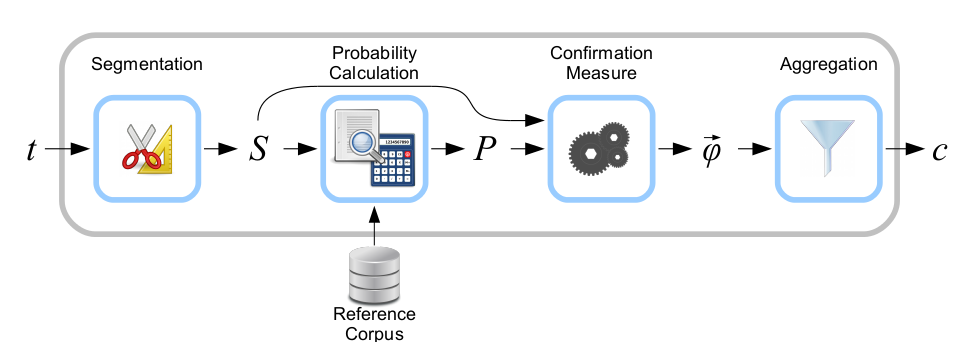
\includegraphics[height=5cm]{images/figure_3.png}
    \caption{Visão geral do framework de mensuração da coerência dos tópicos. Imagem original \citeonline{roder2015exploring}}
\end{figure}


\begin{enumerate}
\item \textbf{Segmentação:} Para cada tópico $t \in \{1 ... K\}$ é extraído um conjunto de palavras mais relevantes de acordo com o modelo resultante,
 então é criado pares combinatórios distintos entre essas palavras. Exemplo:

\begin{table}[h]
  \centering
  \begin{tabular}{l l l l l l l l l}
  & & &0 &1 &2 &3 &4 &5 \\
  \hline
  &Tópico &3 &dados &máquina &mineração &neurais &redes &aprendizagem \\
  \hline
  \end{tabular}
  \caption{Representação de um tópico e suas palavras mais relevantes}
\end{table}

No exemplo acima, vemos um tópico e as palavras com maior probabilidade de pertencerem a ele. É gerado a partir dessas palavras bigramas de palavras $S_i$:

\[\{(m\acute{a}quina, dados),\ (aprendizagem, m\acute{a}quina),\ (neurais, redes),\ ...\}\]

Formalmente é dado por:

\begin{equation}
S_{um}^{um} = \{(W',W^*)|W' = \{w_i\};
W^* =  \{w_j\};w_i,w_j \in W; i \neq j\}
\end{equation}

\begin{equation}
S_{anterior}^{um} = \{(W',W^*)|W' = \{w_i\};
W^* =  \{w_j\};w_i,w_j \in W; i > j\}
\end{equation}

\begin{equation}
S_{posterior}^{um} = \{(W',W^*)|W' = \{w_i\};
W^* =  \{w_j\};w_i,w_j \in W; i < j\}
\end{equation}

As duas últimas são variações da primeira que requer um conjunto ordenado, elas comparam uma palavra apenas com sua palavra anterior e posterior respectivamente, \cite{roder2015exploring}.

\item \textbf{Cálculo de Probabilidade:} É calculado a probabilidade dessas palavras ocorrerem de forma conjunta e pode ser calculado por:

\[P(w_i,w_j) = \frac{N\acute{u}mero\ de\ documentos\ que\ cont\acute{e}m\ palavras\ w_i\ e\ w_j}{Total\ de\ documentos}\]

\item \textbf{Medida de Confirmação:} A medida de confirmação recebe um único par $S_i = (W',W^*)$, ou subconjunto de palavras bem como suas respectivas probabilidades
 para calcular o quão forte o conjunto de palavras condicionais $W^*$ suporta $W'$

\item \textbf{Agregação:} Por fim, todas as confirmações de todos conjuntos de pares $S_i$ são agregados em uma única pontuação de coerência pela sua média.
\end{enumerate}

Nós rodamos o LDA no conjunto de dados com 4, 8, 16, 32, 64 e 128 tópicos e parâmetros $\eta$ e $\alpha$ como distribuições uniformes, para cada configuração de parâmetro $K$,
 obtemos a pontuação de coerência do modelo via processo descrito acima. O valor de $K$ utilizado foi o que obteve maior coerência.

Selecionamos as distribuições do modelo gerado com a configuração de $K$ otimizada, então adicionamos um novo metadado para cada documento armazenado no Elasticsearch com sua distribuição de tópicos.
 Também armazenamos em outra estrutura a distribuição de palavras por tópico. Essas informações serão utilizadas no processo de visualização.

%% APLICAÇÃO
\subsection{APLICAÇÃO}
A aplicação web interativa é uma extensão do LDAVis \cite{sievert2014ldavis}, o trabalho original tem duas funcionalidades principais
que permitem ao usuário explorar o modelo.

\begin{figure}[H]
	\centering
    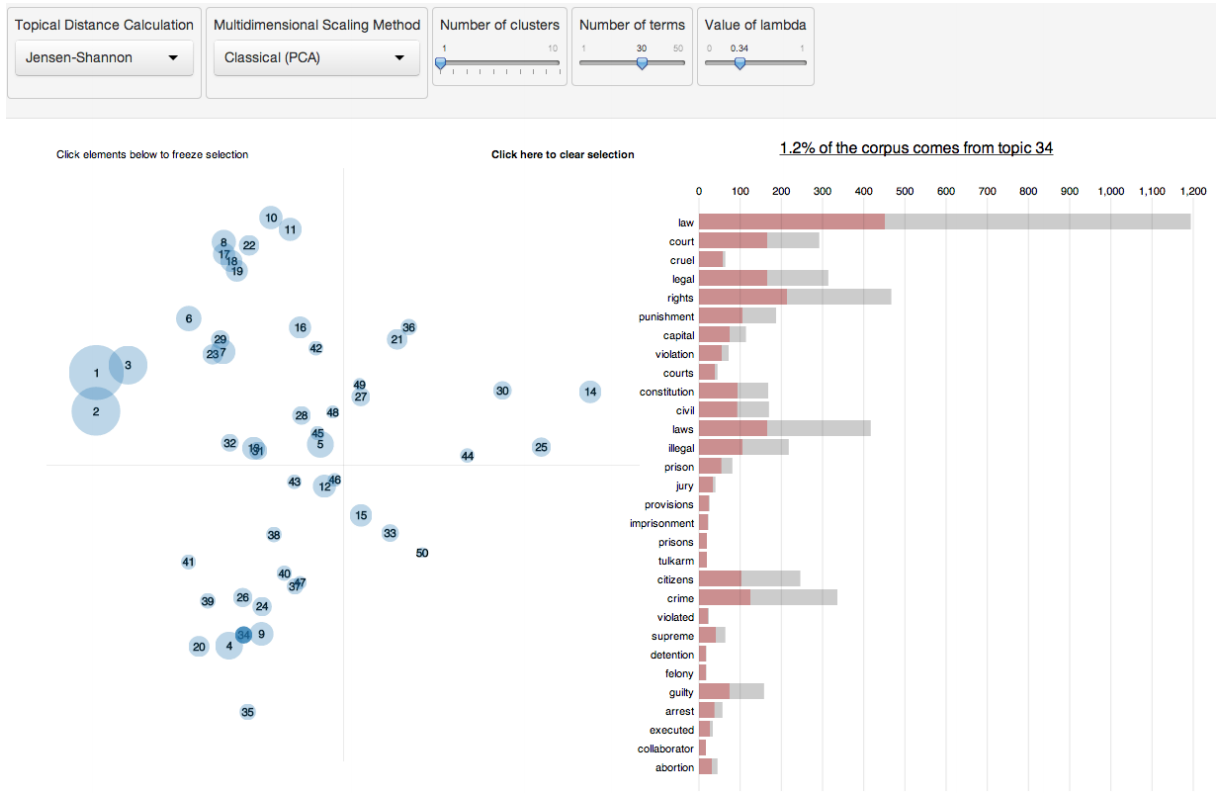
\includegraphics[height=10cm]{images/figure_4.png}
    \caption{Layout do LDAvis. A esquerda a visualização de tópicos e a direita o gráfico de barras com o tópico 34 selecionado. Imagem do trabalho original \cite{sievert2014ldavis}}
\end{figure}


\begin{enumerate}
  \item Possibilita o usuário selecionar um tópico e visualizar os termos mais relevantes dentro dele.
  \item Possibilita o usuário selecionar um termo para revelar sua distribuição condicional sobre os tópicos. Essa distribuição
  é visualizada alterando a área dos círculos tal que seja proporcional a frequência do termo selecionado.
\end{enumerate}

A proposta é estender a visualização para exploração não apenas dos tópicos e palavras mas também dos documentos. Ao final do desenvolvimento esperamos entregar as seguintes funcionalidades extras:

\begin{enumerate}
  \item Busca de documentos:
  \begin{enumerate}
    \item Por palavra.
    \item Por trechos de palavras.
    \item Por data.
    \item Por remetente.
    \item Por destinatários.
    \item Por tópico mais relevante.
  \end{enumerate}
  \item Visualização de comunidades:
  \begin{enumerate}
    \item Por interesse em tópicos comuns.
    \item Por interesse em documentos comuns.
  \end{enumerate}
  \item Análise exploratória do conjunto de dados.
  \begin{enumerate}
    \item Quantidade de documentos por tópico.
    \item Quantidade de usuários.
    \item Usuários mais relevantes por tópico
  \end{enumerate}
\end{enumerate}

Os documentos são indexados e estruturados no Elasticsearch como  descrito na seção 4.1, o próprio motor de busca possui mecanismos para fornecer os tipos de busca e filtros propostos,
 bem como apresentar os dados quantitativos para análise exploratória e criação de comunidades relacionando destinatários e remetentes a seus tópicos frequentes e relevantes.

% Uma comparação entre o modelo LDA e o K-Means será apresentado de forma a demonstrar os benefícios de um modelo misto ao de mistura de unigramas.

%% CRONOGRAMA
\section{CRONOGRAMA}

\begin{center}  
  \begin{tabular}{llllllllll}
                           & Out                    & Nov                    & Dez                      & Jan                    & Fev                    & Mar                     & Abr                    & Mai                     & Jun \\
                           \hline
  Estudo: EM               &\cellcolor[gray]{0.9}   &                        &                          &                        &                        &                         &                        &                         &                        \\
  Qualificação             &                        &\cellcolor[gray]{0.9}   &\cellcolor[gray]{0.9}     &                        &                        &                         &                        &                         &                        \\
  Dev: Modelo              &\cellcolor[gray]{0.9}   &                        &                          &                        &                        &                         &                        &                         &                        \\
  Dev: Buscador            &                        &\cellcolor[gray]{0.9}   &                          &                        &                        &                         &                        &                         &                        \\
  Dev: Expl. Comunidades   &                        &                        &\cellcolor[gray]{0.9}     &                        &                        &                         &                        &                         &                        \\
  Dev: Análise Expl.       &                        &                        &                          &\cellcolor[gray]{0.9}   &                        &                         &                        &                         &                        \\
  Depósito Dissertação     &                        &                        &                          &                        &\cellcolor[gray]{0.9}   &                         &                        &                         &                        \\
  Artigo                   &                        &                        &                          &                        &                        &\cellcolor[gray]{0.9}    &\cellcolor[gray]{0.9}   &\cellcolor[gray]{0.9}    &\cellcolor[gray]{0.9}   \\
  \hline
  \end{tabular}
\end{center}
  

\def\refname{REFERÊNCIAS BIBLIOGRÁFICAS}
\bibliography{biblproj}
\addcontentsline{toc}{section}{REFERÊNCIAS BIBLIOGRÁFICAS}
\bibliographystyle{abnt-alf}

\end{document}
